\hsection{Relationships of a Higher Degree}%
%
\begin{figure}%
\centering%
%
\subfloat[][%
A reproduction of \cref{fig:erdStudentModuleProf3}, which illustrates a ternary relationship of students, modules, and professors with the relationship attribute semester. %
This graphic was painted using \yEd.%
\label{fig:erdStudentModuleProf3B}%
]{\includegraphics[width=0.9\linewidth]{\erdStudentModuleProfIII}}%
%
\floatRowSep%
%
\subfloat[][%
One possible transformation of \cref{fig:erdStudentModuleProf3} to a logical model using \pgmodeler.%
\label{fig:logicalStudentModuleProf}%
]{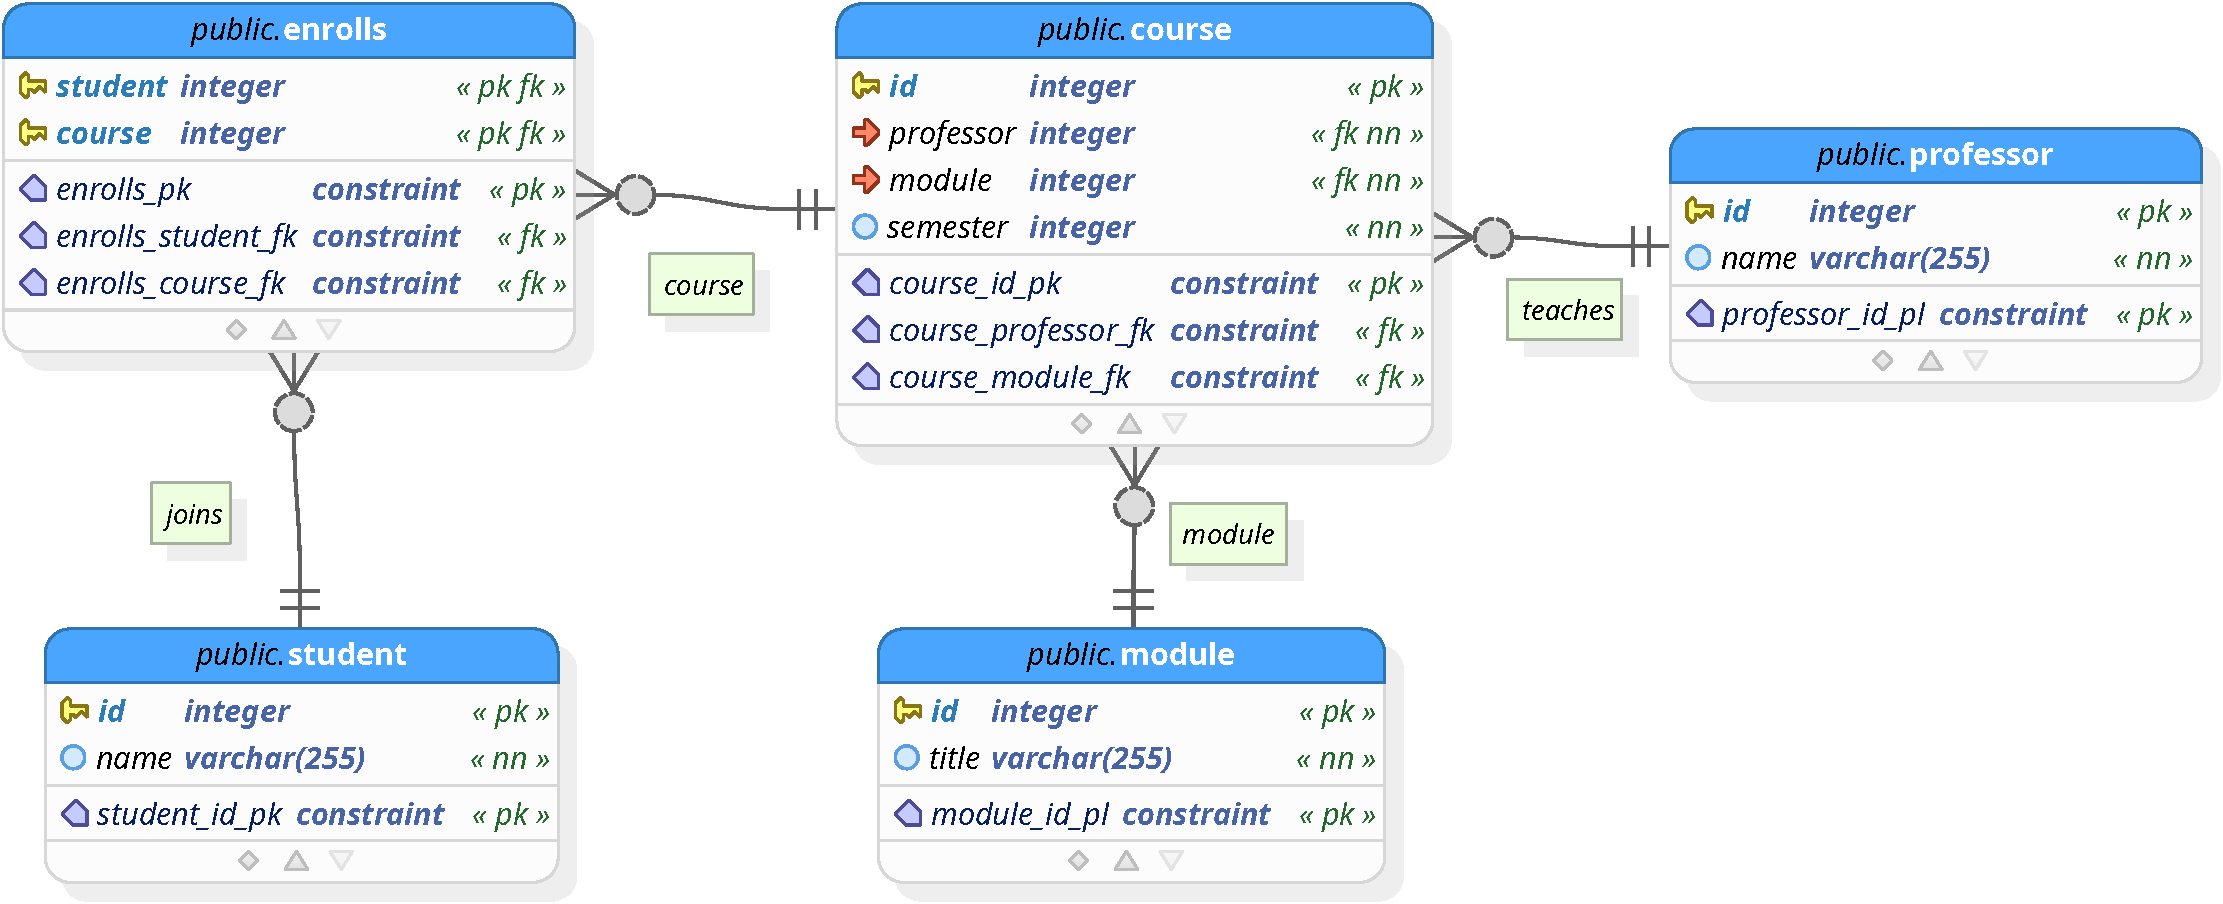
\includegraphics[width=0.9\linewidth]{\currentDir/logicalStudentModuleProf}}%
%
\caption{The representation of relationships with a degree higher than two in relational logical models.}%
\label{fig:logicalStudentModuleProfII}%
\end{figure}%
%
In \cref{fig:erdStudentModuleProf3B}, we reproduce a figure from \dref{sec:conceptual:relationships} where a ternary relationship is illustrated.
The entities \emph{Professor}, \emph{Student}, and \emph{Module} are related with each other and this relationship even has a relationship attribute.
The professor teaches a module in a certain semester.
The student enrolls in that taught module in that semester.

In \cref{fig:logicalStudentModuleProf}, we create a logical model that fits to this scenario.
First, the entities become tables with surrogate primary keys.
We thus get the tables \sqlil{module}, \sqlil{professor}, and \sqlil{student}.
In order to add a bit more sense to this example, we add the attribute \sqlil{name} to the tables \sqlil{student} and \sqlil{professor} as well as \sqlil{title} to \sqlil{module}.

We then construct the ternary relationship.
We basically have two choices to do this:%
%
\begin{enumerate}%
%
\item We can create one single table \sqlil{takes_place} which has three foreign keys to the tables \sqlil{professor}, \sqlil{student}, and \sqlil{module}, as well as a column~\sqlil{semester}.%
%
\item We can create one table~\sqlil{course} with a surrogate key for the \inQuotes{module-instantiation}, which has foreign keys to the tables \sqlil{professor} and \sqlil{module} as well as the column~\sqlil{semester}. %
We create a second table~\sqlil{enrolls} that has two foreign keys, one for the table~\sqlil{student} and one for the table~\sqlil{course}.%
%
\end{enumerate}%
%
Both choices would be feasible, but we go with the second one.
The idea is that we can also consider the realization of a module by a certain professor in a semester as an entity in its own right.
This entity would have the attribute \sqlil{semester}, but could also have arbitrary other attributes that we may want to add later.
Relating the students to that \sqlil{course} table by using a separate table then makes sense.
So we modeled this using \pgmodeler\ and get the logical schema illustrated in \cref{fig:logicalStudentModuleProf}.

\gitSQL{\databasesCodeRepo}{teachingManagement/logical/teaching_database_1/generated_sql/01_teaching_database_database_2001.sql}{teaching_1:01_teaching_database_database_2001}{The generated script to create the \sqlil{teaching_database}~\db.}%
\gitExec{\databasesCodeRepo}{.}{_scripts_/postgres.sh teachingManagement/logical/teaching_database_1/generated_sql 01_teaching_database_database_2001.sql}%
%
\gitSQL{\databasesCodeRepo}{teachingManagement/logical/teaching_database_1/generated_sql/03_public_student_table_5071.sql}{teaching_1:03_public_student_table_5071}{The generated script to create the table~\sqlil{student}.}%
\gitExec{\databasesCodeRepo}{.}{_scripts_/postgres.sh teachingManagement/logical/teaching_database_1/generated_sql 03_public_student_table_5071.sql teaching_database}%
%
\gitSQL{\databasesCodeRepo}{teachingManagement/logical/teaching_database_1/generated_sql/04_public_professor_table_5087.sql}{teaching_1:04_public_professor_table_5087}{The generated script to create the table~\sqlil{professor}.}%
\gitExec{\databasesCodeRepo}{.}{_scripts_/postgres.sh teachingManagement/logical/teaching_database_1/generated_sql 04_public_professor_table_5087.sql teaching_database}%
%
\gitSQL{\databasesCodeRepo}{teachingManagement/logical/teaching_database_1/generated_sql/05_public_module_table_5095.sql}{teaching_1:05_public_module_table_5095}{The generated script to create the table~\sqlil{module}.}%
\gitExec{\databasesCodeRepo}{.}{_scripts_/postgres.sh teachingManagement/logical/teaching_database_1/generated_sql 05_public_module_table_5095.sql teaching_database}%
%
\gitSQL{\databasesCodeRepo}{teachingManagement/logical/teaching_database_1/generated_sql/06_public_course_table_5105.sql}{teaching_1:06_public_course_table_5105}{The generated script to create the table~\sqlil{course} which relates the tables~\sqlil{professor} and~\sqlil{module}.}%
\gitExec{\databasesCodeRepo}{.}{_scripts_/postgres.sh teachingManagement/logical/teaching_database_1/generated_sql 06_public_course_table_5105.sql teaching_database}%
%
\gitSQL{\databasesCodeRepo}{teachingManagement/logical/teaching_database_1/generated_sql/07_public_enrolls_table_5131.sql}{teaching_1:07_public_enrolls_table_5131}{The generated script to create the table~\sqlil{enrolls} which relates the tables~\sqlil{student} and~\sqlil{course}.}%
\gitExec{\databasesCodeRepo}{.}{_scripts_/postgres.sh teachingManagement/logical/teaching_database_1/generated_sql 07_public_enrolls_table_5131.sql teaching_database}%
%
\gitSQL{\databasesCodeRepo}{teachingManagement/logical/teaching_database_1/generated_sql/08_public_course_course_professor_fk_constraint_5116.sql}{teaching_1:08_public_course_course_professor_fk_constraint_5116}{The generated script to create the constraint enforcing that each row in table~\sqlil{course} is related to exactly one row in table~\sqlil{professor}.}%
\gitExec{\databasesCodeRepo}{.}{_scripts_/postgres.sh teachingManagement/logical/teaching_database_1/generated_sql 08_public_course_course_professor_fk_constraint_5116.sql teaching_database}%
%
\gitSQL{\databasesCodeRepo}{teachingManagement/logical/teaching_database_1/generated_sql/09_public_course_course_module_fk_constraint_5117.sql}{teaching_1:09_public_course_course_module_fk_constraint_5117}{The generated script to create the constraint enforcing that each row in table~\sqlil{course} is related to exactly one row in table~\sqlil{module}.}%
\gitExec{\databasesCodeRepo}{.}{_scripts_/postgres.sh teachingManagement/logical/teaching_database_1/generated_sql 09_public_course_course_module_fk_constraint_5117.sql teaching_database}%
%
\gitSQL{\databasesCodeRepo}{teachingManagement/logical/teaching_database_1/generated_sql/10_public_enrolls_enrolls_student_fk_constraint_5145.sql}{teaching_1:10_public_enrolls_enrolls_student_fk_constraint_5145}{The generated script to create the constraint enforcing that each row in table~\sqlil{enrolls} is related to exactly one row in table~\sqlil{student}.}%
\gitExec{\databasesCodeRepo}{.}{_scripts_/postgres.sh teachingManagement/logical/teaching_database_1/generated_sql 10_public_enrolls_enrolls_student_fk_constraint_5145.sql teaching_database}%
%
\gitSQL{\databasesCodeRepo}{teachingManagement/logical/teaching_database_1/generated_sql/11_public_enrolls_enrolls_course_fk_constraint_5151.sql}{teaching_1:11_public_enrolls_enrolls_course_fk_constraint_5151}{The generated script to create the constraint enforcing that each row in table~\sqlil{enrolls} is related to exactly one row in table~\sqlil{course}.}%
\gitExec{\databasesCodeRepo}{.}{_scripts_/postgres.sh teachingManagement/logical/teaching_database_1/generated_sql 11_public_enrolls_enrolls_course_fk_constraint_5151.sql teaching_database}%
%
\gitSQLAndOutput{\databasesCodeRepo}{teachingManagement/logical/teaching_database_1}{insert_and_select.sql}{teaching_database}{}{}{postgres.sh}{teaching_database_1:insert_and_select}{%
Inserting into and selecting data from the tables in the \sqlil{teaching_database}.%
}%
%
\gitExec{\databasesCodeRepo}{.}{_scripts_/postgres.sh teachingManagement/logical/teaching_database_1 cleanup.sql}%
%

Exporting this model \sql\ yields ten scripts.
\Cref{lst:teaching_1:01_teaching_database_database_2001} sets up the \db.
\Cref{lst:teaching_1:03_public_student_table_5071,lst:teaching_1:04_public_professor_table_5087,lst:teaching_1:05_public_module_table_5095,lst:teaching_1:06_public_course_table_5105,lst:teaching_1:07_public_enrolls_table_5131} create the five tables \sqlil{student}, \sqlil{professor}, \sqlil{module}, \sqlil{course}, and~\sqlil{enrolls}, respectively.
\Cref{lst:teaching_1:08_public_course_course_professor_fk_constraint_5116,lst:teaching_1:09_public_course_course_module_fk_constraint_5117,lst:teaching_1:10_public_enrolls_enrolls_student_fk_constraint_5145,lst:teaching_1:11_public_enrolls_enrolls_course_fk_constraint_5151} create the foreign key constraints that ensure referential integrity.

For this purpose, we extend the model further with reasonable assumptions about cardinalities and modalities.
For example, it makes sense to assume that each row in table~\sqlil{course} must be related to exactly one row in table~\sqlil{professor} and exactly one row in table~\sqlil{module}.
We do not permit a course that represents no module of the curriculum and we also do not permit a course that teaches the knowledge of multiple modules at once.
Similarly, we cannot have a course without professor and also we do not permit more than one professor to teach a course.
Well, the latter may actually be possible.
Maybe that would be a good question to bring up during the requirements gathering process or later during conceptual modelling when sitting down with our stakeholders in the university.
At least for now, we do not permit that~(as it would also make our relationship patterns more complicated).

Professors can teach multiple modules and each module can be taught by multiple professors.
We \emph{could} add a \sqlilIdx{UNIQUE} constraint over the combination of the columns~\sqlil{module}, \sqlil{professor}, and~\sqlil{semester}.
This would mean that a professor cannot teach the same module twice in the same semester.
Then again, we can also permit this.
We can easily imagine some \inQuotes{service modules,} like \inQuotes{Mathematics for Engineers,} that many be offered by the School of Mathematics to several other schools, say the School of Computer Science, the School the Engineering, and the School of Agriculture.
Then a professor may offer the same module several times in the same semester, just for different student groups.

We also enforce that each record in the table~\sqlil{enrolls} must relate exactly one row in table~\sqlil{student} and one row in table~\sqlil{course}.
We use the combination of these two foreign keys as primary key.
In other words, no student can enroll in the same course more than once.
Courses are realizations of modules that emerge because a professor teaches them in a specific semester.
So it makes no sense that a student takes part in the same module taught by the same professor in the same semester more than once.
They can, however, take part in the same module in \emph{other} semesters.
Of course, students can also enroll into multiple different courses.

After executing these scripts, we insert some data into the tables in \cref{lst:teaching_database_1:insert_and_select}.
We define the three students Bibbo, Bebbo, and Bebba.
Two professors are declared, namely Weise~(yours truly) and Bobbo.
We enter three modules, namely Python, Databases, and Java.
Via the \sqlil{courses} table, we specify that Prof.~Weise teaches Python and Databases, both in semester~20252, which we interprete as the fall semester in the year~2025.
We also define that Bobbo teaches Java in the spring and fall semesters 2026.

Using four \sqlilIdx{INNER JOIN} expressions, we then merge all the data together.
We order the results by the student name, professor names, module titles, and semesters.
After all of that, we delete the \db\ again using \sqlil{DROP DATABASE}\sqlIdx{DROP!DATABASE}\sqlIdx{DATABASE}.

In this example, we noticed that we could realize the conceptual ternary relationship given in \cref{fig:erdStudentModuleProf3B} in two different ways in a logical schema.
In other scenarios, there may yet be other choices.
It does not make much sense to iterate over all the $\frac{\factorial{(4+3-1)}}{\factorial{(4-1)}*\factorial{3}}=20$ possible ternary relationships here.
Then we would have to also iterate over all 35~possible relationships that involve four entity types, all 56~relationship patterns of five entity types, and so on.
We should also remember that relationship attributes may be present, which could mess up the patterns further.

The somewhat unsatisfying answer on how to implement relationship patterns of more than two entity types is \emph{it depends}.
We are equipped with the ability to enforce referential integrity of arbitrary binary relationship patterns.
We can use this knowledge to reasonably realize patterns that are more complicated.
We just have to build experience.%
\FloatBarrier%
\endhsection%
%
